% acm doc
% https://authors.acm.org/proceedings/production-information/preparing-your-article-with-latex

\documentclass[manuscript]{acmart}

% BUILDING. Do not use ``latex''
% USE
%   brew install mactex
%   cd tex
%   pdflatex -shell-escape vectorio.tex
%   bibtex vectorio
%   ...rerun pdflatex, maybe twice

%\usepackage{babel}
\usepackage{graphicx}
\usepackage{color}
\usepackage{cite}
%\usepackage{algorithmic}
%\usepackage{algorithmicx}
\usepackage[ruled,vlined,boxed]{algorithm2e}
\usepackage{listings}
%\usepackage{minted}
\usepackage{underscore}
\usepackage{multicol}
\usepackage{float}
\usepackage{checkend}
\usepackage{enumitem}


% must come before begin{document}
\citestyle{acmauthoryear}
\setcopyright{none}

\title[Hadoop Vector IO]{Hadoop Vector IO: cloud IO for columnar data formats}

% Yes, this titling is broken
\author{Steve Loughran}
\author{Mukund Thakur}
%  \texttt{mthakur@apache.org}
\author{Owen O'Malley}
%  \texttt{owen@apache.org}

\renewcommand{\shortauthors}{Loughran, et al.}
\date{May 2024}

% ========================================================================

\begin{document}

% ========================================================================

\begin{abstract}
The Hadoop Filesystem API has been extended to support scatter/gather IO
for columnar data formats.
This paper describes the design and implementation of this feature,
and the integration with Apache ORC and Parquet, and
presents results from TPC-DS benchmarks.

Our key findings are that
\begin{itemize}
  \item An asynchronous scatter/gather IO API is ideally suited to retrieval
  of ``stripes''/``row groups'' of data stored in columnar data formats.
  \item Java's native IO APIs support such an API, offering speedups when reading
  local data.
  \item Against cloud storage, the ability to issue parallel GET requests
        significantly improves read performance, providing tangible performance
        improvements to queries which read large quantities of data.
  \item Using the API in the ORC and Parquet is sufficient to enable
        speedups in applications using the libraries \emph{without} any
        changes in the application code.
  \item The API shows that "cloud first" APIs provide tangible speedups
        against the classic Posix API. Many more opportunities exist to
        provide and exploit such APIs.
\end{itemize}

\end{abstract}



\maketitle

% ========================================================================

\section{Introduction}
\label{sec:introduction}



\subsubsection{Terminology}

First, some terminology needs to be introduced to describe
the protocols.

% ========================================================================

\section{The Challenge of Object Stores}
\label{sec:object-stores}

Having introduced the classic filesystem and the commit protocols and algorithms
used to commit the output of distributed computation, let us consider
Object Stores such as Amazon S3, Google Cloud Storage and
Windows Azure Storage.

% As all filesystem
%operations are via the NameNode, all clients get a consistent view of the filesystem.
%And, as the


The most salient point, is this: Object Stores are not filesystems.
Rather than the classic hierarchical view of directories, subdirectories
and paths, object stores store a set of objects, each with a unique key;
a sequence of characters provided when the object was created.
Classic path separators ``\texttt{/}'' are invariably part of the set of valid
characters, so allowing objects to be created which have the appearance
of files in a directory.

As examples, the following are all valid keys on the Amazon, Google and Microsoft
stores

\begin{verbatim}
/entry
/path1/path2/path3
/path1/
/path1
\end{verbatim}

More subtly, it is valid for an object store container (on S3:, a ``bucket'')
to have objects with all of these names simultaneously.
It is not an error to have an object whose key would make it appear to be
``under'' another object, nor to explicitly contain path entries separators.

Objects cannot generally be appended to once created, or renamed.
They can be replaced by new objects or deleted.
Some form of copy operation permits an object to be duplicated, creating
a new object with a different key.
Such copy operations take place within the storage infrastructure with a
copy time measurable in megabytes/second.


The set of operations offered are normally an extended set of HTTP verbs:

\begin{description}[leftmargin=8em, style=nextline]
  \item[PUT] Atomic write of an object
  \item[GET] retrieve all or part of an object
  \item[HEAD] retrieve the object metadata
  \item[LIST] list all objects starting with a given prefix
  \item[COPY] copy a single object within the store, possibly from other containers.
  \item[DELETE] Delete an object
\end{description}

% ========================================================================

\section{Design}
\label{sec:design}

The design of the vector IO API had some core requirements:
\begin{itemize}
  \item Support scatter/gather IO for local filesystem through the java NIO API.
  \item Local reads to support CRC validation of data read if checksum enabled.
  \item Efficient support against cloud stores where parallel GET requests are required.
  \item Support scatter/gather IO through HDFS and other distributed filesystems
        where the POSIX API and Hadoop PositionedReadable interface are available.
  \item Optimize for reading columnar data formats such as ORC and Parquet.
  \item Be easy to integrate with the ORC and Parquet libraries, in the open
        source releases, as well as our own internal branches.
  \item Permit out-of-order result processing, even while the current format libraries
        do not yet support this.
\end{itemize}

What is key is: it \emph{must} be possible to use the vector IO API against
any existing Hadoop input stream, with the base implementation
falling back to the existing \texttt{PositionedReadable} readFully() method,
with the option of custom higher performance implementations --- including
for the local filesystem as well as cloud storage.

Java NIO API:

extending PositionedReadable with range coalescing

Async API with back-references for wiring up.

S3A Impl as ranged GET requests with (limited) parallelism.

\section {Implementation}
\label{sec:implementation}

\subsection{Default implementation}

\begin{quotation}
The default implementation of the vector IO API uses blocking readFully() calls
for each range. This has the same performance as the existing read() API.
\end{quotation}

\subsection{Local/Checksum filesystem implementation}
\begin{quotation}

The local filesystem implementation uses the Java NIO API to read the data
into on-heap buffers in parallel.
\end{quotation}

\subsection{S3A}
\begin {quotation}

S3A implementation of vectored IO coalesces the nearby ranges into a multiple
combined ranges and issues parallel GET requests to AWS S3. Diagram below shows
the full workflow.

\end{quotation}
\begin{figure}
  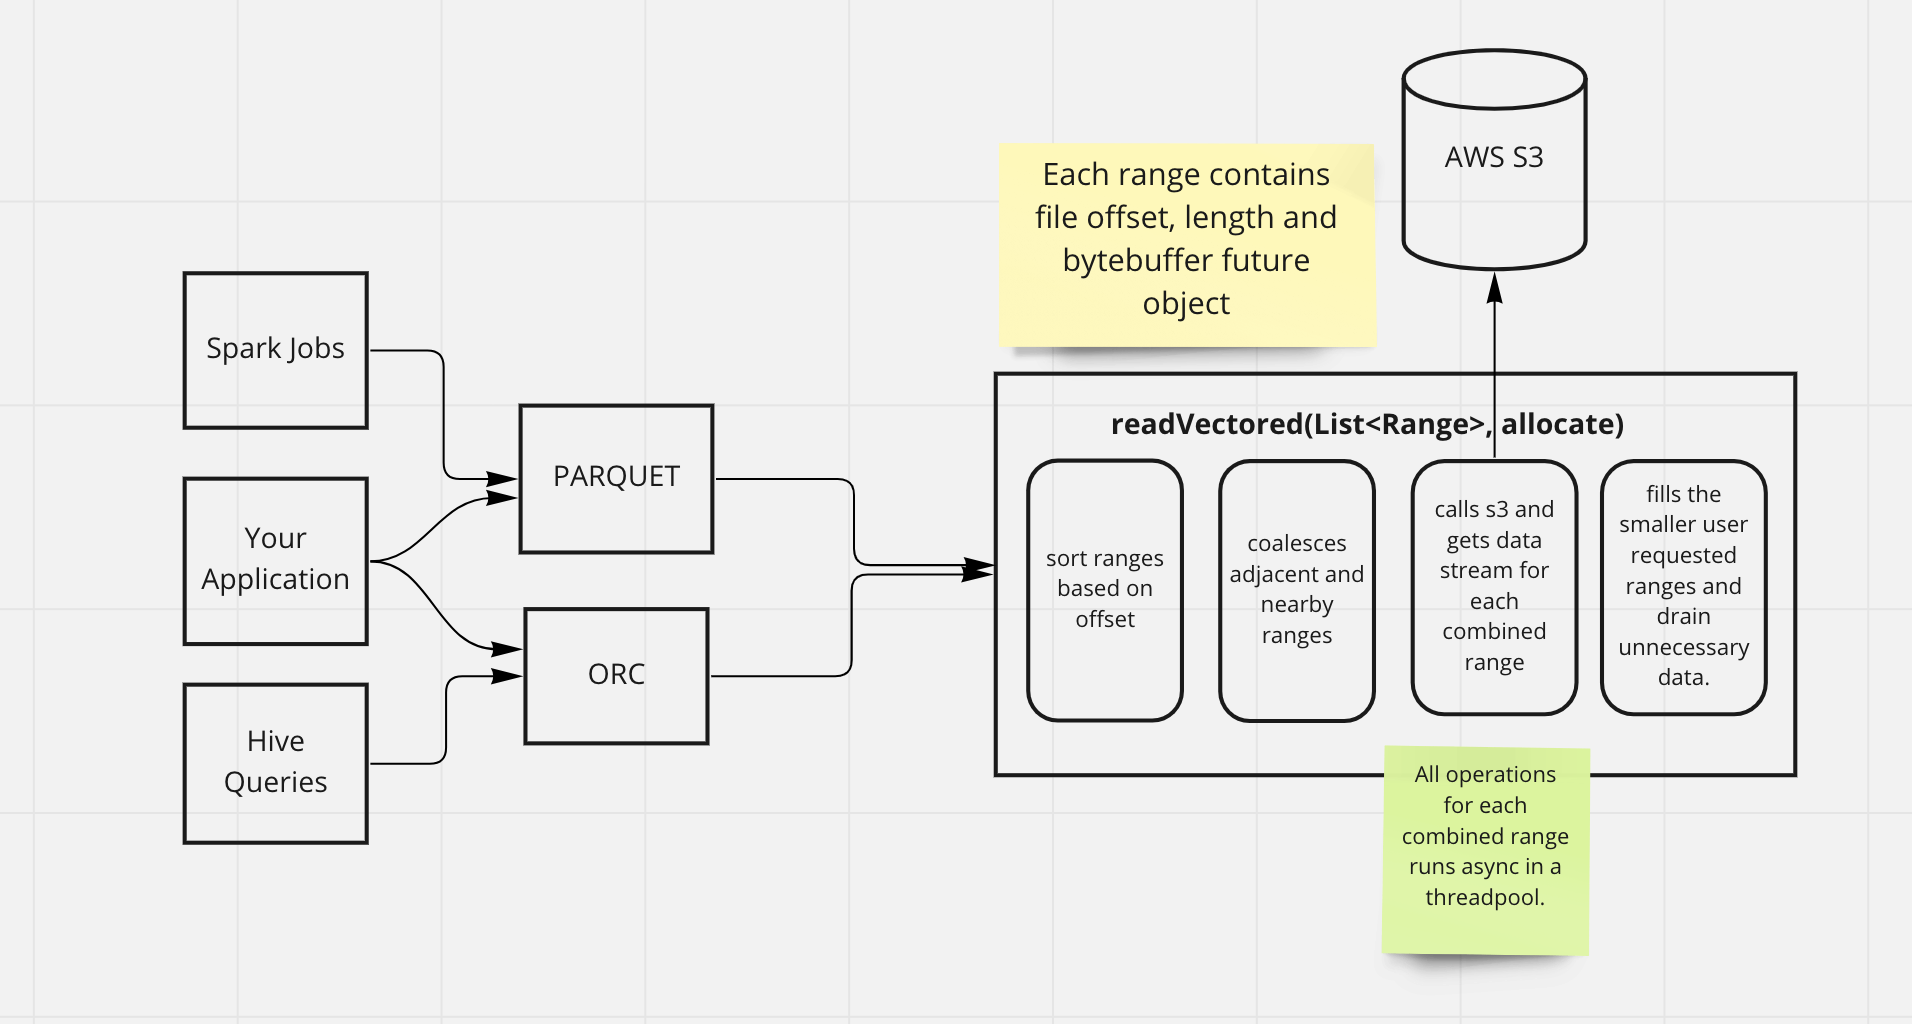
\includegraphics[width=\linewidth]{vectored_io_s3a_flow.png}
  \caption{S3A Vector IO}
  \label{fig:s3a-vector-io}
\end{figure}
% ========================================================================

\section{Integration with ORC and Parquet}
\label{sec:integration}

It was our belief that integration with the ORC and Parquet libraries was
sufficient to deliver tangible speedups
\subsection{ORC}
Apache ORC 2.0.0 implements the vector IO API while reading the multiple disk ranges.
We have been shipping this in our internal releases at Cloudera for some time and will
discuss the performance improvements in the results section.

\subsection{Parquet}
Apache Parquet implements the vector IO API while reading multiple file ranges
and will be shipping in the upcoming 1.14.0 release.
We have been shipping this in our internal releases at Cloudera for some time and will
discuss the performance improvements in the results section.

% ========================================================================

\section{Results}
\label{sec:results}

\subsection{Hive TPC-DS on ORC with Vector IO}
TPC-DS Hive queries with ORC data stored in S3 demonstrated a 10–40\% reduction in
execution time. The data size used was 300 GB in string format. This benchmark was
done on internal cloudera release.
\begin{figure}
  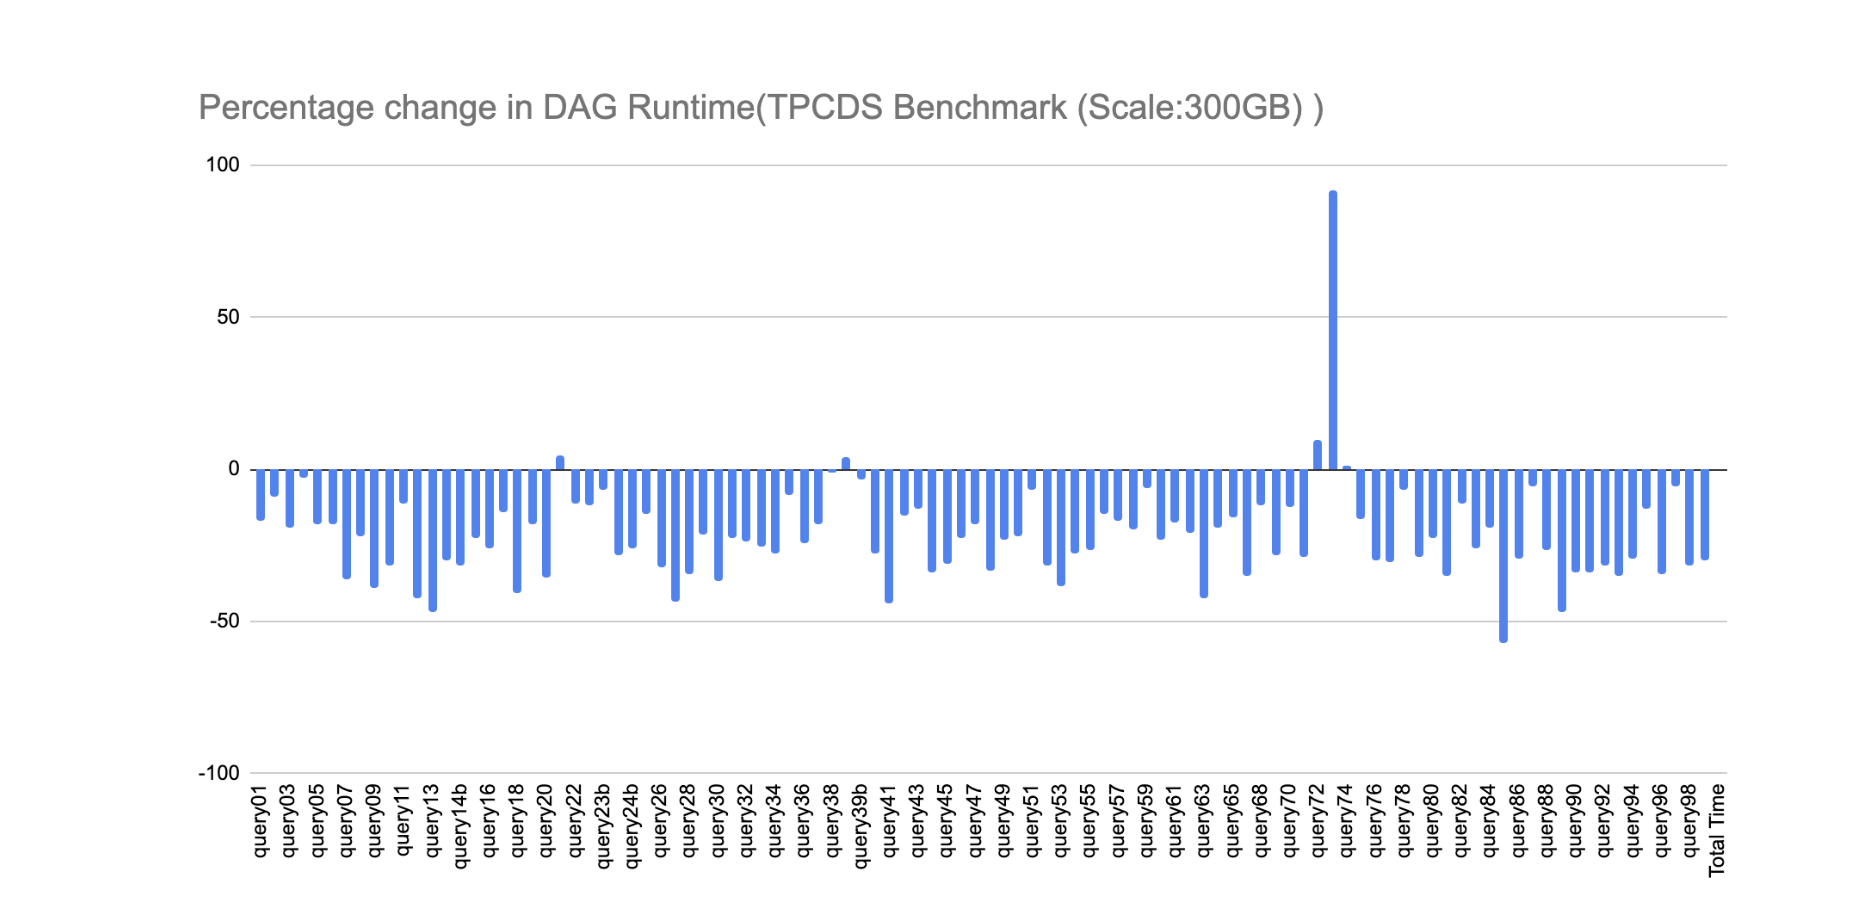
\includegraphics[width=\linewidth]{hive_tpcds_vectored_io.png}
  \caption{Hive TPC-DS on ORC with Vector IO}
  \label{fig:hive_tpcds_vectored_io}
\end{figure}

\subsection{Spark TPC-DS on Parquet with Vector IO}
TPC-DS Spark queries with Parquet data stored in S3 demonstrated a 10–50\% reduction in
execution time. The data size used was 1 TB in string format. This benchmark was
done on internal cloudera release.

\begin{figure}
  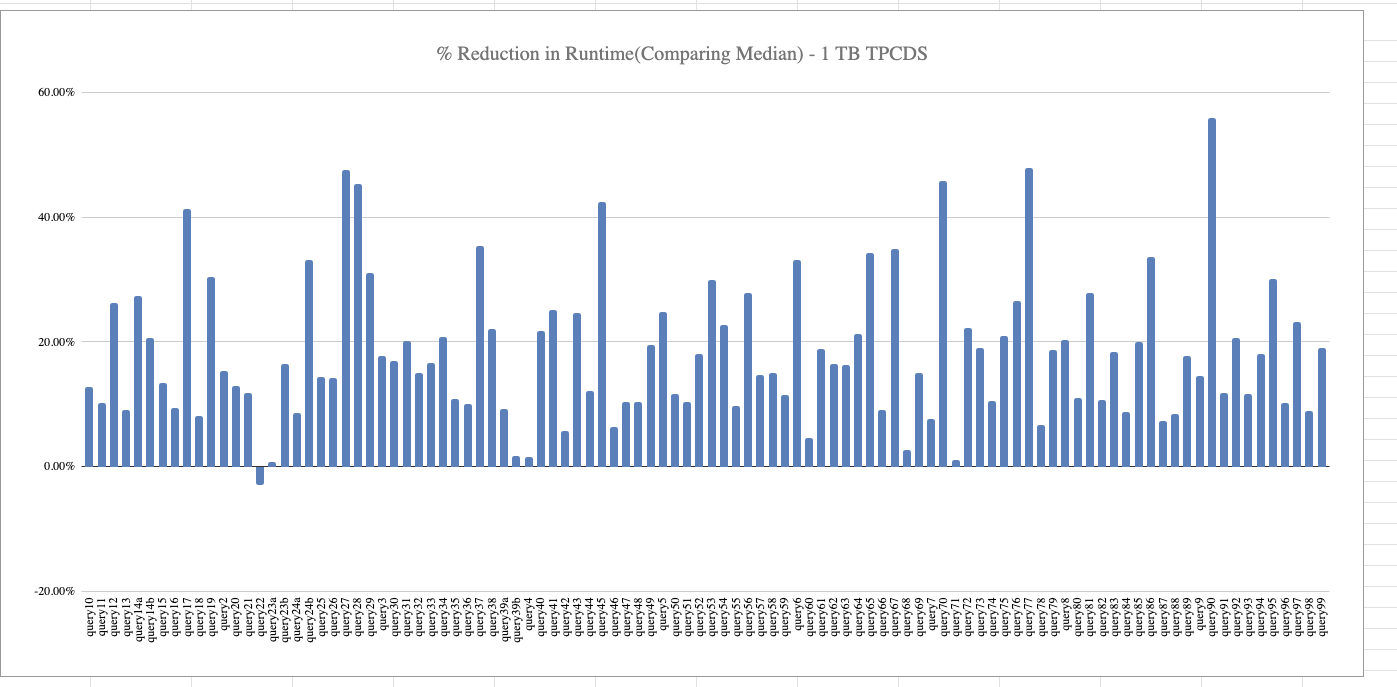
\includegraphics[width=\linewidth]{spark_tpcds_vector_io.png}
  \caption{Spark TPC-DS on Parquet with Vector IO}
  \label{fig:spark_tpcds_vectored_io}
\end{figure}

\subsection{Synthetic ETL benchmark}
%Do we need this here?


\subsection{External tests}

\begin{quotation}
 Some numbers from an independent benchmark.
 I used Spark to parallelize the reading of all rowgroups (just the reading of the raw data)
 from TPC-DS/SF10000/store_sales using various APIs.

I used a modified (lots of stuff removed) version of the ParquetFileReader and a custom
benchmark program that reads all the row groups in parallel and records the time spent in each read from S3.
The modified version of ParquetFileReader can switch between the various methods of reading from S3.
The entry AWS SDK V2 is a near copy of the Iceberg S3FileIO code though.

\end{quotation}

\begin{verbatim}
32 executors, 16 cores
fs.s3a.threads.max = 20
\end{verbatim}

\begin{table}
  \begin{tabular}{ l l l l }
    \hline
    \textbf{Reader} & \textbf{Mean Time/min)} & \textbf{Median} & \textbf{Baseline}\\
    Parquet	& 10.32	& 10 & 1 \\
    Parquet Vector IO	& 2.02 & 2	& 5.1 \\
    SDK V2 & 9.86 & 10 & 1 \\
    SDK V2 Async & 9.66	& 9.6 & 1.1 \\
    SDK V2 AsyncCrt	& 9.76 & 10 & 1.1 \\
    SDK V2 S3TransferManager & 9.58 & 9.5 & 1.1 \\
    SDK V2 Async CRT Http Client & 10.8 & 11 & 1 \\
    \hline
  \end{tabular}
\caption{Independent benchmark results}
\label{tab:independent-benchmark-results}
\end{table}

\begin{quotation}

I saw issues with the CRT client when running at scale causing JVM crashes.
And the V2 transfer manager did not do range reads properly.

Summary - The various V2 SDK clients provide lower latency and better upload speeds but for raw data scans,
they are all pretty much the same.
Increasing the parallelism as vector IO does, has maximum benefit.
\end{quotation}

Analysis.

This benchmark was done with a Hadoop 3.3.x release which had not yet moved to
the AWS SDK V2; this is why the baseline 10:32 time is slower than the "AWS SDK V2"
timing.
Now that Hadoop 3.4.x has moved to the AWS SDK V2, we would expect the v2 timings to
be the default, so the speedups from other methods would not be quite so pronounced.

The AWS V2 SDK includes an "asynchronous client" which is only used by the S3A
connector when copying or uploading files, not when reading them.
The S3TransferManager is the class used to manage these operations.
The "CRT http client" is a native C library to which the SDK can delegate much
of the work of building, signing, sending and receiving HTTP requests, and processing
the responses.

Although the CRT promises speedups, our experience with using openssl instead of
the Java JRE's open TLS implementation makes us wary of the potential for
unusual failure conditions which may occur in some deployments.

For the open source hadoop releases, moving to the "Async" client is something
which could be done with lower risk; switching to CRT library would then be
an optional which could be explicitly enabled in deployments.

% ========================================================================

\section{Limitations}
\label{sec:limitations}

% ========================================================================

\section{Related Work}
\label{sec:related-work}

\section{Conclusions and Further Work}
\label{sec:conclusions}

\subsubsection{Multi-ranged GET requests}.

The HTTP protocol allows for a client to request multiple ranges of a file
in the same request.
If supported by cloud object stores, this will allow for a single request
over a single HTTP connection to retrieve different row groups in the same
request, \emph{irrespecive of their location in the file}.
This would assist coalescing range requests, reduce the number of HTTP requests
needed while avoiding the need to discard data between ranges.

\subsubsection{Footer prefetching and cacheing}

As shown in \cite{zeng2023empirical}, and in our own analyisis of trace data
obtained from audit logs of storage systems, reading the footer date of ORC and Parquet
files can be a significant cost.

When these files are first opened, the initial read sequence is

\begin{itemize}
  \item{open the file}
  \item{read the final 8 bytes to validate filetype and the offset for the "real" footer}
  \item{read the full footer}
\end{itemize}

On HDFS the costs of this are
\begin{itemize}
  \item{namenode: open the file}
  \item{read the final 8 bytes to validate filetype and the offset for the "real" footer}
  \item{read the full footer}
\end{itemize}






% ========================================================================

\begin{acks}
We are grateful for the contributions of all reviewers and testers of this work,
especially our fellow developers in the open source community,
especially Dongjoon Hyun, Parth Chandra, and Gang Wu.
Special mention must be made of the Cloudera QE team whose scale testing
not only produced the numbers in this paper, but also identified a large number
of regressions related unrelated changes in the S3A codebase (move to AWS v2 SDK).
As much of that work was contributed by Mukund and Steve, we are grateful.
\end{acks}


% ========================================================================

\section{References}
\label{sec:references}

% Bibliography. Include

\bibliographystyle{ACM-Reference-Format}
\bibliography{bibliography}



\appendix{}

\section{Appendix}
We like to introspect and review what problems actually occurred
in production.
This helps us review our assumptions, consider how valid they proved
to be, and to let us analyze how they got through our reviews and testing.
Hopefully others can learn from our mistakes.


\subsection{HADOOP-19101. Vectored Read into off-heap buffer broken in fallback implementation}
\label{HADOOP-19101}

Default implementation reads into Direct (off JVM-heap buffer reads broken.
This surfaced when adding tests for azure storage.
Our previous tests against the local and S3 stores used custom implementations
which were correct. Lesson: always test those defaults.
This has never been seen ``in the wild'' because the applications
using the library do not seem to be reading into Direct buffers.
As well as fixing the bug, the integration patch for Parquet reports all
attempt to use vectored IO with Direct buffers as ``unsupported''.
This ensures that even when using old releases, the bug will not surface.

\end{document}
